\chapter{Capital Structure}
\section{Introduction}
\begin{itemize}
    \item Learn how the firm chooses a mix of debt-to-equity.
    \item Assume a perfect capital markets world, but later add taxes and the risk of financial distress.
    \item This chapter will determine the effects of taxes and financial distress on the optimal capital structure.
    \item This chapter also discusses the trade-off theory and finding the optimal debt-to-equity ratio.
\end{itemize}

\section{The Modigliani and Miller Theorem (Case 1)}

\begin{figure}[H]
    \centering
    \begin{tikzpicture}
        % Define styles for blocks and labels
        \tikzstyle{assetblock} = [rectangle, draw, fill=cyan!50, text width=5cm, text centered, minimum height=4cm, inner sep=0pt, outer sep=0pt]
        \tikzstyle{equityblock} = [rectangle, draw, fill=green!50, text width=5cm, text centered, minimum height=2cm, inner sep=0pt, outer sep=0pt]
        \tikzstyle{debtblock} = [rectangle, draw, fill=gray!50, text width=5cm, text centered, minimum height=2cm, inner sep=0pt, outer sep=0pt]
        \tikzstyle{labelstyle} = [rectangle, text centered, inner sep=0pt, outer sep=0pt]
        
        % Draw the Asset block
        \node[assetblock] (assets) at (0,0) {$V = A$ \\ $R_A$ \\ $\beta_A$};
        \node[labelstyle, above=of assets] (assetslabel) {Assets};
        
        % Draw the Equity and Debt blocks
        \node[equityblock] (equity) at (5,1) {$E = \text{Equity}$\\$R_E$\\ $\beta_E$};
        \node[debtblock, below=0 of equity] (debt) {$D = \text{Debt}$\\$R_D$\\ $\beta_D$};
        \node[labelstyle, above=of equity] (equitydebtlabel) {Equity and Debt};
        
        % Label column setup
        \node[labelstyle] at (assetslabel) {Assets};
        \node[labelstyle] at (equitydebtlabel) {Equity and Debt};
    \end{tikzpicture}
    \caption{Diagram illustrating the structure of assets, equity, and debt.}
    \label{fig:assets_equity_debt}
\end{figure}

\begin{itemize}
    \item The left-hand side has net operating assets and the right-hand side represents sources of financing. 
    \item In this simple model, as there are no taxes or risk of financial distress, cash flows generated by the firm from its net operating assets are independent of the sources of funding (capital structure). 
    \item \textbf{The firm's value is not affected by the financing method}. 
    \item The free cash flows are easily distributed to the debt and equity holders.
\end{itemize}

\begin{definitionbox}{WACC in Case 1 (No Tax and No Risk of Financial Distress)}
    \begin{equation}
        R_A = WACC = \frac{E}{D+E} \cdot R_E + \frac{D}{D+E} \cdot R_D
    \end{equation}
\end{definitionbox}

$R_A$ is the unlevered assets return as there are no taxes.

\begin{itemize}
    \item As debt is cheaper than debt, it's easy to assume to increasing leverage and taking on more debt will lower the cost of capital and increase the value of the firm.
    \item But how does this reconcile with the fact that cash flows are independent of financing?
    \item This is described by the Modigliani and Miller Theorem, which says as we acquire more debt capital, the equity becomes riskier, leading to a higher rate of return demanded by equity holders, and the cost of equity increases.
    \item So this offsets the benefit of cheaper debt, and the cost of capital remains the same.
\end{itemize}

\begin{theorembox}{Modigliani and Miller Theorem}
    \begin{enumerate}
        \item \textbf{Proposition one: } the firm's value is unaffected by the capital structure, as cash flows are independent of financing sources.
        \item \textbf{Proposition two: } the cost of capital is not influenced by the capital structure.
        
    \end{enumerate}
    \begin{align}
        R_A &= WACC= \frac{E}{D+E} \cdot R_E + \frac{D}{D+E} \cdot R_D\\
        \Rightarrow \underbrace{R_E}_{\text{Cost of Equity Capital}} &= \underbrace{R_A}_{\text{Unlevered Cost of Capital}} + \underbrace{\frac{D}{E} \cdot (R_A - R_D)}_{\text{Risk premium that is increasing on the debt-to-equity ratio}}
    \end{align}

    This is because we can express the cost of equity as a variable that is increasing in the debt-to-equity ratio.\\

    We can express the $\beta_E$, or the equity beta, in a similar manner.
    \begin{align}
        \beta_A &= \frac{E}{D+E} \cdot \beta_E + \frac{D}{D+E} \cdot \beta_D\\
        \Rightarrow \underbrace{\beta_E}_{\text{Equity Beta}} &= \underbrace{\beta_A}_{\text{Business Risk or Unlevered Beta}} + \underbrace{\frac{D}{E} \cdot (\beta_A - \beta_D)}_{\text{Risk premium that is increasing on the debt-to-equity ratio}}
    \end{align}
\begin{itemize}
    \item Equity beta ($\beta_E$) represents the risk of a firm's equity, accounting for its level of leverage. It is derived from the unlevered beta ($\beta_A$), which is the beta of the firm without debt, and adjusted (adding an extra risk-premium ratio) based on the firm's debt-to-equity ratio. 

    \item As leverage (debt-to-equity ratio) increases, the equity beta ($\beta_E$) also increases, indicating a higher risk associated with the equity of the firm. This is because the risk of default and financial distress increases with more debt, placing a higher risk premium on the equity.
\end{itemize}

\end{theorembox}

\begin{examplebox}{Example}
    Suppose we set up a firm that operates for one period and needs to reaise \$1000. Consider two capital structures:

    \begin{figure}[H]
        \centering
        \begin{tabular}{lccc}
        \toprule
        Economic Condition & Firm Earnings & All Equity Case & 50\% Debt Finance ($R_D = 5\%$) \\
        \midrule
        Good economy (50\%) & 14 (+40\%)   & 14 (+40\%)      & 17.5 (+75\%) \\
        Bad economy (50\%)  & 9 (-10\%)    & 9 (-10\%)       & 7.5 (-25\%) \\
        \bottomrule
        \end{tabular}
        \caption{Comparison of firm earnings in different economic conditions and financing scenarios}
    \end{figure}
    

    \begin{itemize}
        \item 100\% equity financing
        \item 50-50 debt-equity financing
    \end{itemize}

    Firm's performance depends on the state of the economy, let's assume it can be either strong or weak with the same probability 50-50.

\begin{itemize}
    \item For the fully-equity financed firm, all the operating income goes to equity holders
    \item The all-equity case will give a return of 14 in a good economy and 9 in a bad economy, translating to a 40\% increase in a good economy and a 10\% decrease in a bad economy.
    \item In the mixed capital structure, some of the income is used to pay off debt holders. This increases the return in a good economy to 17.5, a 75\% increase, and decreases the return in a bad economy to 7.5, a 25\% decrease.
    \item Notice how much more volatile the returns of a 50-50 debt-equity financed firm are compared to the all-equity financed firm. It has almost effectively doubled.
    \item This is why equity holders will demand more returns given the risk.
    \item The WACC for the all-equity firm given both states of the economy is 15\%, netting a positive expected return.
    \item The WACC for the 50-50 debt-equity firm is 25\%, so even though there is a risk of a more negative return, the expected return is higher than the all-equity financed firm.
    \begin{align}
        WACC_{\text{All Equity}} = R_E &= \frac{E}{D+E} \cdot R_E + \frac{D}{D+E} \cdot R_D \\
                                       &= 0.5 \times (40\%) + 0.5 \times (-10\%) = 15\%\\
        WACC_{\text{50-50 Debt-Equity}} = R_E &= \frac{E}{D+E} \cdot R_E + \frac{D}{D+E} \cdot R_D\\
                                        &= 0.5 \times (75\%) + 0.5 \times (-25\%) = 25\%
    \end{align}

\end{itemize}

\end{examplebox}

\begin{figure}[H]
    \centering
    \includegraphics[width=0.7\textwidth]{img/8.2.png}
    \caption{Graph visualisation of the cost of capital over debt-to-value ratio}
\end{figure}

$r_{WACC}$, or the weighted average cost of capital, is constant regardless of the capital structure. This is because the increase in the debt cost of capital offsets the gain from cheaper financing. The red and blue lines sum together to form the yellow line.


\section{Modigliani and Miller's Theorem in a more realistic world (Case 2)}

We now incorporate taxes into our model (case 2), which are tax deductible. This means that the cost of debt is reduced by the tax shield.

\begin{enumerate}
    \item We could use the WACC method that assumes a constant debt-to-equity ratio as the firm grows, and reduce the cost of debt in proportion to the corporate tax rate $\tau_c$.
    \item Another method is the adjusted present value method, more flexible, and does not assume a constant debt-to-equity ratio. It involves calculating the unlevered value of the firm as if it were all equity-financed, and then discounting expected tax savings over time using an appropriate cost of capital.
\end{enumerate}


\subsection*{WACC method for calculating the cost of capital}
\begin{definitionbox}{WACC in Case 2 (With Corporate Tax and No Risk of Financial Distress)}
    For the WACC method, the WACC be expressed as such (note in some equations, $V = D + E$ is used in the denominator):

\begin{align}
    WACC &= \underbrace{\frac{E}{D+E} \cdot R_E}_{\text{Cost of Equity Weighted}} + \underbrace{\frac{D}{D+E} (1-\tau_C) \cdot R_D}_{\text{After-Tax Cost of Debt Weighted}}\\
         &= \underbrace{\frac{E}{D+E} \cdot R_E + \frac{D}{D+E} \cdot R_D}_{\text{Let this be }R_U \text{in the case of D=0}}\ - \ \tau_C \cdot \frac{D}{D+E} \cdot R_D\\
         &= \underbrace{R_U}_{\text{Unlevered Cost of Capital (assuming 100\% equity structure)}} - \underbrace{\tau_C \cdot \frac{D}{D+E} \cdot R_D}_{\text{Reduction due to tax shield}}
\end{align}

\end{definitionbox}

We discount the tax shield by $(1-\tau_C)$, where $\tau_C$ is the corporate tax rate. This is because interest payments are tax-deductible, so the tax shield is the interest payment multiplied by the tax rate.\\

$R_U$ is required return rate on equity for unleveraged firm, taking the case of $D=0$ and thus $R_U = R_E$.\\

This implies cost of equity can be expressed as the unlevered cost of capital plus the difference between the unlevered cost of capital and the cost of debt.

\begin{figure}[H]
    \centering
    \includegraphics[width=0.7\textwidth]{img/8.3.png}
    \caption{Graph visualisation of the cost of capital over debt-to-value ratio with taxes}
\end{figure}

The issue with this model now is that we are now incentivised to maximise debt without limits, because the corporate tax rate is a fixed discount rate, so we can go all out on debt and reduce the cost of capital indefinitely.

This is where the third case comes in, incoporating the risk of financial distress. 

\begin{examplebox}{True or False?}
\begin{enumerate}
    \item When capital markets are perfect, the portfolio of a firm’s equity and debt replicates the returns we would earn if the firm were unlevered. \textbf{True}
    \item If we can identify a comparison firm whose assets have the same risk as the firm being evaluated, and if the comparison firm is levered, then we can use its equity cost of capital as the cost of capital for our evaluation. \textbf{False}
    
    \item We can calculate the cost of capital of the firm’s assets by computing the weighted average of the firm’s equity and debt cost of capital, which we refer to as the firm’s Weighted Average Cost of Capital (WACC). \textbf{True}
    
    \item When estimating the market value of a firm’s asset, we must use a discount rate that is appropriate given the risk of the firm’s free cash flow. \textbf{True}
\end{enumerate}
\end{examplebox}
\begin{examplebox}{Ungeared vs Geared Firm}
    \textbf{Question 1:} Consider two firms, Geared and Ungeared, that have identical assets that generate identical cash flows. Assume no taxes and no risk of default. Ungeared is an all-equity firm, with 1 million shares outstanding, which trade for a price of \$24 per share. Geared has 2 million shares outstanding and \$12 million dollars in debt at an interest rate of 5\%. If there is no opportunity for capital arbitrage, the stock price for Geared will be:
    
    \textbf{Answer:} \$6.00
    

    \begin{align*}
    \text{Total value of Ungeared} &= 1,000,000 \times \$24 = \$24,000,000 \\
    \text{Total debt of Geared} &= \$12,000,000 \\
    \text{Total equity value of Geared} &= \$24,000,000 - \$12,000,000 = \$12,000,000 \\
    \text{Number of shares of Geared} &= 2,000,000 \\
    \text{Stock price for Geared} &= \frac{\$12,000,000}{2,000,000} = \$6.00
    \end{align*}
    
    \textbf{Question 2:} If Ungeared has a cost of equity capital of 10\%, what is the cost of equity capital of the Geared firm?
    

    
    Let \( R_E \) be the cost of equity capital for the Ungeared firm, and \( R_E' \) be the cost of equity capital for the Geared firm. The cost of equity capital for the Geared firm can be calculated as follows:\\

    Using the Modigliani-Miller theorem:
    \begin{align*}
    R_E' &= R_E + (R_E - R_D) \left(\frac{D}{E}\right) \\
         &= 10\% + (10\% - 5\%) \left(\frac{\$12,000,000}{\$12,000,000}\right) \\
         &= 10\% + 5\% = 15\%
    \end{align*}
    
\end{examplebox}

\begin{examplebox}{Canton Corporation Financial Analysis}
    \textbf{Question:} The unlevered cost of capital for Canton Corporation is 10\%. The firm is financed with 30\% debt that offers a promised return of 15\% and has an expected return of 8\%. Canton is in the 40\% marginal tax bracket.
    
    \textbf{What is Canton's WACC?}
    
    \textit{Answer:}
    \begin{align*}
   \text{WACC} &= R_U - \tau_c \frac{D}{V} R_D \\
               &= 10\% - 0.4 \times 0.3 \times 8\% \\
               &= 10\% - .96\% = 9.04\%
    \end{align*}

    (For WACC, we use only expected return on debt, not the promised return.)
    
    \textbf{What is Canton’s expected cost of equity financing?}
    
    \textit{Answer:} 
    \begin{align*}
        R_E &= R_A + \frac{D}{E} (R_A - R_D) \\
            &= 10\% + \frac{0.3}{0.7} (10\% - 8\%) \\
            &= 10.86\%
    \end{align*}
\end{examplebox}


\begin{examplebox}{Analysis of Change in Capital Structure}
    \textbf{Question:} Your firm has a before-tax return of \$1,800 on an investment of \$800 and a marginal tax rate of 25\%. The unlevered cost of capital is 10\%. The firm currently uses 30\% debt financing with an expected return of 7\%. If it increases its use of debt to 40\%, the expected return on the debt will be 8\%.
    
    \textbf{Calculate your firm's WACC under the current capital structure.}
    
    \textit{Answer:}
    \begin{align*}
    \text{WACC} &= R_U - \tau_c \frac{D}{V} R_D \\
               &= 10\% - 0.25 \times 0.3 \times 7\% \\
               &= 10\% - 0.525\% = 9.48\%
    \end{align*}
    
    \textbf{Calculate your firm's WACC under the proposed capital structure.}
    
    \textit{Answer:}
    \begin{align*}
    \text{WACC} &= R_U - \tau_c \frac{D}{V} R_D \\
               &= 10\% - 0.25 \times 0.4 \times 8\% \\
               &= 10\% - 0.8\% = 9.2\%
    \end{align*}
\end{examplebox}
    







\subsection*{Adjusted Present Value (APV) method}
\begin{sidenotebox}{APV Method}
    The Adjusted Present Value (APV) approach is used to value a firm by considering the effects of debt separately from the operating assets. The APV method can be particularly useful in scenarios where the capital structure is complex or changing. The APV is calculated as follows:

\begin{align}
    APV &= V_U + PV(\text{Tax Shield}) \\
    V_U &= \sum_{t=1}^{T} \frac{FCF_t}{(1 + R_U)^t}
\end{align}

Where:
\begin{itemize}
    \item \( V_U \) is the value of the unlevered firm (i.e., the firm if it had no debt).
    \item \( FCF_t \) is the free cash flow to the firm at time \( t \).
    \item \( R_U \) is the unlevered cost of capital.
    \item \( T \) is the number of periods.
    \item \( PV(\text{Tax Shield}) \) is the present value of the tax shield due to debt.
\end{itemize}


\subsection*{Calculating the Present Value of the Tax Shield}

The tax shield can be calculated using the corporate tax rate \( \tau_C \) and the debt \( D \) as follows:

\begin{align}
    PV(\text{Tax Shield}) &= \tau_C \cdot D \cdot \frac{1 - (1 + R_D)^{-T}}{R_D}
\end{align}

Where:
\begin{itemize}
    \item \( R_D \) is the cost of debt.
    \item \( D \) is the total amount of debt.
    \item \( \tau_C \) is the corporate tax rate.
    \item \( T \) is the number of periods the debt is held.
\end{itemize}

\subsection*{Advantages of APV}

The APV method allows for the flexibility of adjusting the valuation for different financing scenarios. It is especially useful when:
\begin{itemize}
    \item The firm's capital structure is changing over time.
    \item The risk profile of debt is different from that of the firm’s assets.
\end{itemize}

\subsection*{Comparison to WACC}

Unlike the WACC method, which requires an assumption of a constant target capital structure, APV separates the value of the firm into components. This separation can provide more clarity in situations where the financing mix is not stable or predictable.
\end{sidenotebox}

\section{Live Class: Capital Structure in Practice (Case 3)}
In the Live Class, Diageo is analysed as an example to find the right balance between debt and equity.
\subsection*{Diageo Case Study}

\begin{itemize}
    \item Diageo is one of the largest food and drink companies in the world.
    \item Initially, it had three main businesses: 
    \begin{enumerate}
        \item Alcoholic beverages
        \item Packaged Foods
        \item Fast food restaurants
    \end{enumerate}
    \item In the 2000s, there were major changes in the core business:
    \begin{enumerate}
        \item Selling their packaged food subsidiary (Pillsbury) to General Mills for \$5.1 billion in cash plus 141 million shares of General Mills (about 33\% of Market Cap)
        \item Spin-off of Burger King
        \item A lot changed on the left-hand side (Assets) of the Balance Sheet; a good opportunity to optimise the right-hand side (Debt and Equity Financing) as well – historically conservative (See \ref{fig:assets_equity_debt} for balance sheet diagram.)
    \end{enumerate}
\end{itemize}


\subsection*{Optimum Capital Structure}
\begin{theorembox}{Trade-Off Theory}
    The trade-off theory of capital structure suggests that firms have a target capital structure that balances the benefits of debt (such as tax shields and lower cost of capital) with the costs of debt (such as financial distress and agency costs). The optimal capital structure is the one that maximises the firm's value by balancing these trade-offs.
\end{theorembox}


\begin{figure}[H]
    \centering
    \begin{subfigure}{0.55\textwidth}
        \centering
        \includegraphics[width=\textwidth]{img/8.4.1.png}
        \caption{The Weighted Average Cost of Capital}
    \end{subfigure}

    \begin{subfigure}{0.55\textwidth}
        % \centering
        % \includegraphics[width=\textwidth]{img/8.4.2.png}
        % \caption{Firm Value and the Optimum Capital Structure}
        \centering
        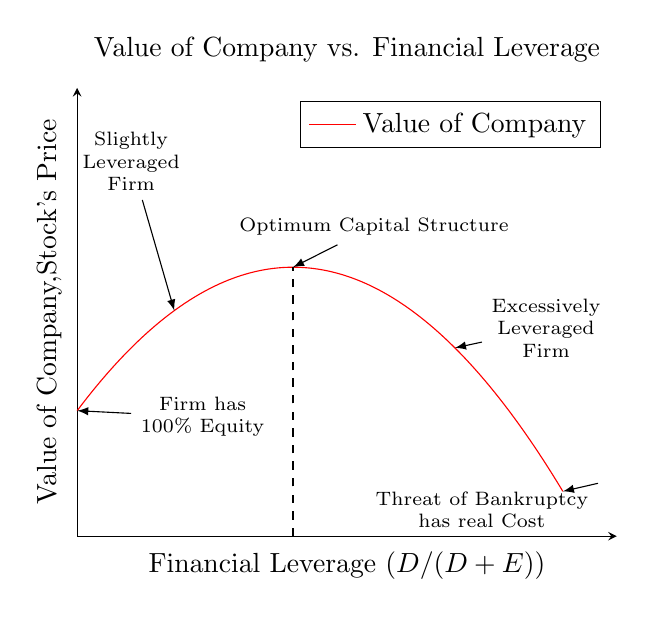
\begin{tikzpicture}
        \begin{axis}[
            title={Value of Company vs. Financial Leverage},
            xlabel={Financial Leverage (\( D / (D+E) \))},
            ylabel={Value of Company,Stock's Price},
            xmin=0, xmax=1,
            ymin=0, ymax=100,
            xtick=\empty, xticklabels={},
            ytick=\empty, yticklabels={},
            legend pos=north east,
            grid style=dashed,
            axis lines = left,
            clip=false,
        ]
        
        % Adding the parabolic curve
        \addplot[
            domain=0:0.9, 
            samples=100, 
            color=red,
        ]
        {-200*(x-0.4)^2 + 60};
        \addlegendentry{Value of Company}
        
    % Nodes with connecting arrows
    \node (sl) at (axis cs:0.1,75) [anchor=south, font=\scriptsize, align=center] {Slightly \\ Leveraged\\ Firm};
    \draw[-latex] (sl) -- (axis cs:0.18,50.32);
    
    \node (ex) at (axis cs:0.75,55) [anchor=north west, font=\scriptsize, align=center] {Excessively \\ Leveraged\\ Firm};
    \draw[-latex] (ex) -- (axis cs:0.7,42);
    
    \node (eq) at (axis cs:0.1,20) [anchor=south west, font=\scriptsize, align=center] {Firm has \\100\% Equity};
    \draw[-latex] (eq) -- (axis cs:0,28);
    
    \node (bn) at (axis cs:0.75,12) [anchor=north, font=\scriptsize, align=center] {Threat of Bankruptcy\\ has real Cost};
    \draw[-latex] (bn) -- (axis cs:0.9,10);

    \node (op) at (axis cs:0.55, 65) [anchor=south, font=\scriptsize, align=center] {Optimum Capital Structure};
    \draw[-latex] (op) -- (axis cs:0.4,60);
    
    % Adding dashed lines for visual aid
    \draw[dashed] (axis cs:0.4,0) -- (axis cs:0.4,60);
    
    
        % Adding dashed lines for visual aid
        \draw[dashed] (axis cs:0.4,0) -- (axis cs:0.4,60);
        
        \end{axis}
        \end{tikzpicture}
        \caption{The relationship between financial leverage and company value, showing the optimum capital structure.}
    \end{subfigure}
    \caption{Graphs showing the optimum point of capital structure}
\end{figure}


\subsection*{Leveraged Recapitalisation}
Leveraged recapitalisation is a strategy used by companies to increase their debt levels and reduce their equity levels. This can be done by issuing debt and using the proceeds to buy back shares or pay a special dividend to shareholders. This increases leverage while maintaining the same share price. 

\begin{figure}[H]
    \centering
    \includegraphics[width=0.7\textwidth]{img/8.4.3.png}
    \caption{Diagram of Leveraged Recap}
\end{figure}

\subsection*{Before the Recap}
\begin{itemize}
    \item Assets: \$3.5M
    \item Financing (100\% Equity): \$3.5M
    \item Discount Rate: 20\%
    \item Tax Rate: 30\%
    \item Interest Rate: 10\%
\end{itemize}


Income Statement:
\[
\begin{array}{lr}
    \text{EBIT} & 1,000,000 \\
    \text{- Taxes} & 300,000 \\
    \hline
    \text{= Net income} & 700,000 \\
\end{array}
\]


Net income is \$700K.
To get \$3.5M:

\begin{align*}
    \$ 3,500,000 = \sum^{\infty}_{t=1}\frac{\$700,000}{1.2^t} = \frac{\$700,000}{.2}
\end{align*}


\subsection*{After the Recap}
\begin{itemize}
    \item Assets: \$3.5M + Tax Shield: (\$0.3M)  
    \item Financing: \$3.8M (\$2.8M Equity, \$1M Debt)
\end{itemize}

Income Statement:
\[
\begin{array}{lr}
    \text{EBIT} & 1,000,000 \\
    \text{- Interest} & 100,000 \\
    \text{Taxable Income} & 900,000 \\
    \text{- Taxes} & 270,000 \\
    \hline
    \text{= Net income} & 630,000 \\
\end{array}
\]

The annual tax shield is $\$300,000-\$270,000 = \$30,000$.

To calculate value of the firm (\$3.8M):
\begin{align*}
 \$ 3,800,000 &= \sum^{\infty}_{t=1} {\frac{\$700,000}{1.2^t}} + \sum^{\infty}_{t=1} {\frac{\$30,000}{1.1^t}}\\
   &= \frac{\$700,000}{0.2} + \frac{\$30,000}{0.1} = \$3,800,000
\end{align*}

We discount using 1.1 for the tax shield, because it is the discount rate minus the interest rate

\subsection*{What Happens to the Share Price?}

\subsubsection*{Before the Recap}
\begin{itemize}
    \item Assets: \$3.5M
    \item Financing (100\% Equity): \$3.5M
\end{itemize}

\subsubsection*{After the Recap}
\begin{itemize}
    \item Assets: \$3.5M + Tax Shield: (\$0.3M)  
    \item Financing: \$3.8M (\$2.8M Equity, \$1M Debt)
\end{itemize}

Assume $m=1M$ shares outstanding before recap.

\begin{itemize}
    \item $P_0 = \$3.5$ (Before Recap)
    \item Share buyback. Let's say we have $D=\$1M$ to buy back at $p=\$3.5$ per share. 
    \item We will buy $n$ shares. So $n = 1M/3.5 = 285,714$ shares.
    \item After the buyback:
    \begin{itemize}
        \item Equity Value = \$630,000
        \item \# of shares outstanding = 714,286
        \item New share price = \$2.8M/0.714M = \$3.92
    \end{itemize}
\end{itemize}

We have to choose a $p$ such that shareholders are willing to tender their shares.

\begin{itemize}
    \item $np = D$ where $D$ is the debt we raise to buy back shares.
    \item $np = \$1M$
    \item $(m-n)p = E$ where $E$ is the equity value after the buyback.
    \begin{align*}
        mp - np &= E \\
        \$p \times 1M - \$1M &= \$2.8M \\
        p &= \$3.8
    \end{align*}
    \item $n = \$1M/\$3.8 = 263,158$
\end{itemize}

\subsection*{Taking on Too Much Debt, Costs of Financial Distress}
\begin{itemize}
    \item If the firm loses money, it cannot get the tax deduction
    \item This will negatively affect operations, causing economic distress
    \item Leads to agency problems
    \item Direct impact on bankruptcy costs (bankruptcy costs are a function of the amount of debt)
\end{itemize}

\begin{table}[h]
    \centering
    \caption{S\&P Credit Ratings with Average EBIT/Interest and Debt/Capital Ratios. A rating of BBB and higher is considered investment grade, while ratings below BBB are considered speculative.}
    \label{tab:credit_ratings}
    \begin{tabular}{lll}
    \toprule
    \textbf{Rating} & \textbf{Avg. EBIT/Interest} & \textbf{Average Debt/Capital (\%)} \\
    \midrule
    AAA & 12.9 & 21.4 \\
    AA  & 9.2  & 29.3 \\
    A   & 7.2  & 33.3 \\
    BBB & 4.1  & 40.8 \\
    \midrule
    \addlinespace 
    BB  & 2.5  & 55.3 \\
    B   & 1.2  & 68.8 \\
    CCC & -0.9 & 71.5 \\
    \bottomrule
    \end{tabular}
\end{table}

\subsection*{Should Diageo Increase Leverage?}

\subsubsection*{Diageo Case Study Recap}

\begin{itemize}
    \item Diageo is one of the largest food and drink companies in the world.
    \item Initially, it had three main businesses: 
    \begin{enumerate}
        \item Alcoholic beverages
        \item Packaged Foods
        \item Fast food restaurants
    \end{enumerate}
    \item In the 2000s, there were major changes in the core business:
    \begin{enumerate}
        \item Selling their packaged food subsidiary (Pillsbury) to General Mills for \$5.1 billion in cash plus 141 million shares of General Mills (about 33\% of Market Cap)
        \item Spin-off of Burger King
        \item A lot changed on the left-hand side (Assets) of the Balance Sheet; a good opportunity to optimise the right-hand side (Debt and Equity Financing) as well – historically conservative (See \ref{fig:assets_equity_debt} for balance sheet diagram.)
    \end{enumerate}
\end{itemize}

\subsubsection*{Debt}
\begin{itemize}
    \item \textbf{Tax Shield: }
    \begin{itemize}
        \item Low/high tax rate? 27\%
        \item Tax Loss Carry Forwards: This is a tax provision that allows companies to carry forward losses to future years to offset profits and reduce tax liability.
        \item UK new cap to tax shield: a worldwide group can deduct against its taxable profits to a maximum of 30\% of taxable EBITDA. In other words, the tax shield is limited to 30\% of EBITDA.
        \item Do any other tax credits exist? For example, R\&D. But Diageo does not have them
    \end{itemize}
    \item \textbf{Discipline/Governance: }
    \begin{itemize}
        \item Does Diageo have governance issues?
        \item How is its free cash flow?
    \end{itemize}
    \item \textbf{Risk: }
    \begin{itemize}
        \item Debt cyclicality: Low/high? Current beta on debt is 0.55
        \item Volatility: How is the stability of its cash flows?
        \item Any technological risk? A technological risk could be a new competitor entering the market with a new technology that disrupts the industry. In Diageo's case, none.
        \item Competition risk? Yes, Diageo has many competitors.
        \item Currency risk? Yes, Diageo has currency risk as it is a global company.
        \item Legal risk? Possibly, as it operates in multiple countries, has many brands (risk of IP disputes), and sells alcohol, is large (risk of antitrust and competition law)
        \item Regulation risk? Yes, Diageo is in the alcohol industry, which can be subject to alcohol regulations, marketing restrictions, taxation and duty increases, health and safety regulations, ethics etc.
    \end{itemize}
    \item \textbf{Distress Costs:}
    \begin{itemize}
        \item Investment Needs: Diageo is large, can benefit from economies of scale, possible to grow via organic growth, and M\&A. Can invest in new products/markets/talents/R\&D.
        \item Assets: Mostly low tech tangibles. Intangibles include brand value. 
        \item Competition: High competition, aggressive market players. 
        \item Customers: Will customers stop buying if Diageo is in distress? Does it have a durable competitive advantage?
        \item Employees: The business is human-capital intensive, in R\&D, marketing, process.
        \item Management: Is management capable of managing a highly leveraged firm?
    \end{itemize}
\end{itemize}

\subsection*{Diageo's Checklist}
\subsubsection*{Pros}
\begin{itemize}
    \item Tax-shield?
    \item Governance/Discipline?
\end{itemize}
\subsubsection*{Cons}
\begin{itemize}
    \item Are cash flows risky? Hard to hedge?
    \item What if they got into financial distress?
    \item Financial flexibility?
    \item Liquidity of assets, hard to value/sell/redeploy in the event of a crisis?
    \item Rivals more aggresive?
    \item Customers/Suppliers care?
    \item Employees care?
    \item Management capable?
\end{itemize}

\subsection*{60\% D/A Recap: Value Impact}

Before the recapitalization is announced:
\begin{itemize}
    \item Market equity \( E_{\text{pre-recap}} = £20.144M \)
    \item Debt \( D_{\text{pre-recap}} = £6,882M \)
    \item Firm value \( V_{\text{pre-recap}} = £27,026M \)
\end{itemize}

After the recapitalization is implemented:
\begin{itemize}
    \item Tax shield created \( \text{PVTS} \approx t \times \text{New } D = 30\% \times 418 = £125M \)
    \item Firm value \( V_{\text{post-recap}} = £27,026M + 125M = £27,151M \)
    \item Debt \( D_{\text{post-recap}} = £6,882M + 418M = £7,300M \)
    \item Market equity \( E_{\text{post-recap}} = £27,151M - 7,300M = £19,851M \)
\end{itemize}

Market equity drops but shareholders are better off as overall they get:
\[
E_{\text{at announcement}} = \text{Payout} + E_{\text{post-recap}} = 418M + 19,851M = £20,269M
\]

\subsection*{60\% D/A Recap: Transaction}

\begin{itemize}
    \item Pre-recap, there are 3,397M shares.
    \item Stock price reaction to the recap announcement:
    \begin{itemize}
        \item Stock price pre-recap: £5.93
        \item Stock price at announcement: \( \frac{£20,269M}{3,397M} = £5.97 \)
    \end{itemize}
    \item Diageo repurchases \( \frac{418M}{5.97} = 70M \) shares.
    \item Remaining shares post-recap: \( 3,397M - 70M = 3,327M \) shares.
    \item Stock price post recap: \( \frac{£19,851M}{3,327M} = £5.97 \)
\end{itemize}

\subsection*{Analysis of Recap Values}
\begin{figure}[H]
    \centering
    \includegraphics[width=0.95\textwidth]{img/8.4.4.png}
    \caption{Comparison of recap amounts. A higher 70\% D/A amount causes a higher share price, but reduces debt rating and earnings per share.}
\end{figure}

\section{The Private Equity Debate: Podcast}
\subsection*{FOR Private Equity}

\begin{enumerate}
    \item Private equity firms outperform on an operating basis, demonstrating their ability to create value for their investors.
    \item The outperformance of private equity firms, even after accounting for fees, suggests that they are doing something substantial.
    \item Private equity investments provide diversification benefits, as shown by studies comparing them to public stock portfolios.
    \item Dividend recapitalisations, enabled by low interest rates, offer a legitimate way to return value to investors and discipline management.
\end{enumerate}

\subsection*{AGAINST Private Equity}

\begin{enumerate}
    \item Private equity returns may not be as impressive when accounting for the risk involved, particularly due to high leverage.
    \item Private equity firms often mark their own inventory, potentially inflating their performance figures and masking risks.
    \item The practice of selling companies to other private equity firms, rather than strategic buyers, raises questions about the actual value creation.
    \item Some studies indicate that private equity ownership may lead to negative outcomes for society, such as increased mortality rates in certain industries.
    \item Dividend recapitalisations may artificially boost returns without necessarily indicating genuine value creation or company improvement.
\end{enumerate}

